%  LaTeX support: latex@mdpi.com
%  In case you need support, please attach all files that are necessary for compiling as well as the log file, and specify the details of your LaTeX setup (which operating system and LaTeX version / tools you are using).

% You need to save the "mdpi.cls" and "mdpi.bst" files into the same folder as this template file.

%=================================================================
\documentclass[electronics,article,submit,moreauthors,pdftex,10pt,a4paper]{mdpi}
\synctex=1
\usepackage{fixme}
\usepackage{caption}
\usepackage{subcaption}
\usepackage{listings}             % Include the listings-package
\usepackage{placeins}
\usepackage{xcolor}
\usepackage{caption}
\usepackage{textcomp}  % To get the correct quotes in lstlistings (')

\newcommand\floor[1]{\left\lfloor#1\right\rfloor}
\newcommand\ceil[1]{\left\lceil#1\right\rceil}

\newcommand{\todot}[1]{%
  \textcolor{red}{TODO: #1}
}

%--------------------
% Class Options:
%--------------------
% journal
%----------
% Choose between the following MDPI journals:
% actuators, admsci, aerospace, agriculture, agronomy, algorithms, animals, antibiotics, antibodies, antioxidants, applsci, arts, atmosphere, atoms, axioms, batteries, behavsci, beverages, bioengineering, biology, biomedicines, biomimetics, biomolecules, biosensors, brainsci, buildings, carbon, cancers, catalysts, cells, challenges, chemosensors, children, chromatography, climate, coatings, computation, computers, condensedmatter, cosmetics, cryptography, crystals, data, dentistry, designs, diagnostics, diseases, diversity, econometrics, economies, education, electronics, energies, entropy, environments, epigenomes, fermentation, fibers, fishes, fluids, foods, forests, futureinternet, galaxies, games, gels, genealogy, genes, geosciences, geriatrics, healthcare, horticulturae, humanities, hydrology, informatics, information, infrastructures, inorganics, insects, instruments, ijerph, ijfs, ijms, ijgi, inventions, jcdd, jcm, jdb, jfb, jfmk, jimaging, jof, jintelligence, jlpea, jmse, jpm, jrfm, jsan, land, languages, laws, life, literature, lubricants, machines, magnetochemistry, marinedrugs, materials, mathematics, mca, mti, medsci, medicines, membranes, metabolites, metals, microarrays, micromachines, microorganisms, minerals, molbank, molecules, mps, nanomaterials, ncrna, neonatalscreening, nutrients, particles, pathogens, pharmaceuticals, pharmaceutics, pharmacy, philosophies, photonics, plants, polymers, processes, proteomes, publications, recycling, religions, remotesensing, resources, risks, robotics, safety, sensors, separations, sexes, sinusitis, socsci, societies, soils, sports, standards, sustainability, symmetry, systems, technologies, toxics, toxins, universe, urbansci, vaccines, vetsci, viruses, water
%---------
% article
%---------
% The default type of manuscript is article, but can be replaced by:
% addendum, article, book, bookreview, briefreport, casereport, changes, comment, commentary, communication, conceptpaper, correction, conferencereport, expressionofconcern, meetingreport, creative, datadescriptor, discussion, editorial, essay, erratum, hypothesis, interestingimage, letter, newbookreceived, opinion, obituary, projectreport, reply, retraction, review, sciprints, shortnote, supfile, technicalnote
% supfile = supplementary materials
%----------
% submit
%----------
% The class option "submit" will be changed to "accept" by the Editorial Office when the paper is accepted. This will only make changes to the frontpage (e.g. the logo of the journal will get visible), the headings, and the copyright information. Also, line numbering will be removed. Journal info and pagination for accepted papers will also be assigned by the Editorial Office.
%------------------
% moreauthors
%------------------
% If there is only one author the class option oneauthor should be used. Otherwise use the class option moreauthors.
%---------
% pdftex
%---------
% The option pdftex is for use with pdfLaTeX. If eps figure are used, remove the option pdftex and use LaTeX and dvi2pdf.

% *** ACRONYM PACKAGE ***
\usepackage[nolist]{acronym}
% \acf{GS} writes Ground Station
% \ac{GS} writes GS exept for the first time
%syntax: \acro{<acronym>}[<short name>]{<full name>}
\begin{acronym}[]
\acro{3GPP}{3rd Generation Partnership Project}
\acro{ACK}{Acknowledgment}
\acro{AMR}{Adaptive Multi-Rate}
\acro{AP}{Access Point}
\acro{ARQ}{Automatic Repeat-reQuest}
\acro{ARF}{Auto Rate Fallback}
\acro{API}{Application Programming Interface}
\acro{BER}{Bit Error Rate}
\acro{BLAS}{Basic Linear Algebra Subprograms}
\acro{BS}{Base Station}
\acro{BSS}{Basic Service Set}
\acro{cdf}{Cummulative Density Function}
\acro{CFP}{Contention Freeze Periode}
\acro{CPU}{Central Processing Unit}
\acro{CSMA/CA}{Carrier Sense Multiple Access with Collision Avoidance}
\acro{CW}{Contention Window}
\acro{CWN}{Cooperative Wireless Network}
\acro{CTS}{Clear to Send}
\acro{D2D}{Device to Device}
\acro{DAG}{Direct Acyclic Graph}
\acro{DCF}{Distributed Coordination Function}
\acro{DIFS}{Distributed Interframe Space}
\acro{ERP}{Extended Rate PHY}
\acro{FEC}{Forward Error Correction}
\acro{FCS}{Frame Check Sequence}
\acro{FF}{Finite Field}
\acro{GF}{Galois Field}
\acro{GPS}{Global Positioning System}
\acro{GPU}{Graphic Processing Unit}
\acro{HTTP}{Hyper Text Transfer Protocol}
\acro{IBSS}{Independent BSS}
\acro{IC}{Interference Cancellation}
\acro{ICST}{Institute for Computer Sciences, Social-Informatics and Telecommunications Engineering}
\acro{IFS}{Interframe Space}
\acro{IoT}{Internet of Things}
\acro{IP}{Internet Protocol}
\acro{IPTV}{Internet Protocol TeleVision}
\acro{JCN}{Journal of Communications and Networks}
\acro{KL}{Kullback-Leibler}
\acro{LAN}{Local Area Network}
\acro{l.d.}{linearly dependent}
\acro{l.i.}{linearly independent}
\acro{LNC}{Linear Network Coding}
\acro{LOS}{Line Of Sight}
\acro{LTE-A}{Long Term Evolution Advanced}
\acro{MAC}{Medium Access Control}
\acro{MANET}{Mobile Ad hoc NETwork}
\acro{MIMO}{Multiple Input Multiple Output}
\acro{MIT}{Massachusetts Institute of Technology}
\acro{MTBF}{Mean Time Between Failure}
\acro{M2M}{Machine-to-Machine}
\acro{NAV}{Network Allocation Vector}
\acro{NEP}{Nokia Energy Profiler}
\acro{NC}{Network Coding}
\acro{NLOS}{Non Line Of Sight}
\acro{NIC}{Network Interface Card}
\acro{OSI}{Open Systems Interconnect}
\acro{PC}{Personal Computer}
\acro{PDA}{Personal Digital Assistant}
\acro{PEP}{Packet Error Probability}
\acro{pgf}{Probability Generating Function}
\acro{PHY}{Physical Layer}
\acro{PLCP}{Physical Layer Convergence Procedure}
\acro{pmf}{Probability Mass Function}
\acro{PNC}{Physical layer Network Coding}
\acro{PPDU}{PLCP Protocol Data Unit}
\acro{QoS}{Quality of Service}
\acro{RLNC}{Random Linear Network Coding}
\acro{ROC}{Region of Convergence}
\acro{SRLNC}{Sparse Random Linear Network Coding}
\acro{SIMD}{Single Instruction Multiple Data}
\acro{SAIC}{Single Antenna Interference Cancellation}
\acro{SIFS}{Short Interframe Space}
\acro{SIMD}{Single Instruction Multiple Data}
\acro{SINR}{Signal-to-Interference-plus-Noise Ratio}
\acro{SMP}{Symmetric Multiprocessor}
\acro{SNMP}{Simple Network Management Protocol}
\acro{SNR}{Signal-to-Noise Ratio}
\acro{SOC}{System on Chip}
\acro{SSE}{Streaming SIMD Extensions}
\acro{SSID}{Service Set Identifier}
\acro{TSNC}{Tunable Sparse Network Coding}
\acro{UDP}{User Datagram Protocol}
\acro{UML}{Unified Modeling Language}
\acro{UI}{User Interface}
\acro{VANET}{Vehicular Ad-hoc Network}
\acro{VoIP}{Voice over Internet Protocol}
\acro{WBN}{Wireless Broadcast Network}
\acro{WiFi}{Wireless Fidelity}
\acro{WLAN}{Wireless Local Area Network}
\acro{WMN}{Wireless Mesh Network}
\acro{pmf}{Probability Mass Function}
\acro{TC}{Telescopic Codes}
\acro{TBTT}{Target Beacon Transmision Times}
\acro{TCP}{Transmission Control Protocol}
\acro{dof}{degrees of freedom}
\acro{IP}{Internet Protocol}
\acro{OS}{Operating System}
\acro{NFS}{Network File System}
\acro{RAM}{Random Access Memory}
\end{acronym}
 % Name of acronyms file

% *** ALGORITHM PACKAGE ***
\usepackage[]{algorithm2e}

% *** PDF PACKAGE *** ..to extract a page from a PDF with multiple pages.
\usepackage{pdfpages}

%=================================================================
\firstpage{1}
\makeatletter
\setcounter{page}{\@firstpage}
\makeatother
\articlenumber{x}
\doinum{10.3390/------}
\pubvolume{xx}
\pubyear{2016}
\copyrightyear{2016}
\externaleditor{Academic Editor: Steven Johnston and Simon J. Cox}
\history{Received: date; Accepted: date; Published: date}
%------------------------------------------------------------------
% The following line should be uncommented if the LaTeX file is uploaded to arXiv.org
%\pdfoutput=1

%=================================================================
% Add packages and commands here. The following packages are loaded in our class file: fontenc, calc, indentfirst, fancyhdr, graphicx, lastpage, ifthen, lineno, float, amsmath, setspace, enumitem, mathpazo, booktabs, titlesec, etoolbox, amsthm, hyphenat, natbib, hyperref, footmisc, geometry, caption, url, mdframed

%=================================================================
%% Please use the following mathematics environments:
 \theoremstyle{mdpi}
 \newcounter{thm}
 \setcounter{thm}{0}
 \newcounter{ex}
 \setcounter{ex}{0}
 \newcounter{re}
 \setcounter{re}{0}

 \newtheorem{Theorem}[thm]{Theorem}
 \newtheorem{Lemma}[thm]{Lemma}
 \newtheorem{Corollary}[thm]{Corollary}
 \newtheorem{Proposition}[thm]{Proposition}

 \theoremstyle{mdpidefinition}
 \newtheorem{Characterization}[thm]{Characterization}
 \newtheorem{Property}[thm]{Property}
 \newtheorem{Problem}[thm]{Problem}
 \newtheorem{Example}[ex]{Example}
 \newtheorem{ExamplesandDefinitions}[ex]{Examples and Definitions}
 \newtheorem{Remark}[re]{Remark}
 \newtheorem{Definition}[thm]{Definition}
%% For proofs, please use the proof environment (the amsthm package is loaded by the MDPI class).

%=================================================================
% Full title of the paper (Capitalized)
\Title{Easy as Pi: A Network Coding Raspberry Pi Testbed}

% Authors, for the paper (add full first names)
\Author{Chres W. S{\o}rensen $^{1,\dagger}$*, N\'estor J. Hern\'andez Marcano $^{1,2,\dagger}$, Juan A. Cabrera G. $^{3,4}$, Simon Wunderlich $^{3}$, Daniel E. Lucani $^{1,\dagger}$ and Frank H. P. Fitzek $^{3}$}
% Authors, for metadata in PDF
\AuthorNames{Chres W. Soerensen, Nestor J. Hernandez M., Juan Cabrera, Simon Wunderlich, Daniel E. Lucani and Frank H. P. Fitzek}
% Affiliations / Addresses (Add [1] after \address if there is only one affiliation.)
\address{%
$^{1}$ \quad Aalborg University, Department of Electronic Systems. Aalborg, Denmark; \{cws, nh, del\}@es.aau.dk\\
$^{2}$ \quad Steinwurf ApS. Aalborg, Denmark; nestor@steinwurf.com\\
$^{3}$ \quad Technische Universit\"at Dresden, Deutsche Telekom Chair of Communication Networks. Dresden, Germany; \{juan.cabrera, frank.fitzek\}@tu-dresden.de, simon.wunderlich@mailbox.tu-dresden.de\\
$^{4}$ \quad SFB 912 -- Collaborative Research Center HAEC. Dresden, Germany}

% Contact information of the corresponding author
\corres{Correspondence: cws@es.aau.dk; Tel.: +45 99 40 87 23}
%\corres{Correspondence: nestor@steinwurf.com, nh@es.aau.dk; Tel.: +45 51 20 03 49}

% Current address and/or shared authorship
\firstnote{Fredrik Bajers Vej 7A, Room A3-110. Aalborg, Denmark}

% Simple summary
%\simplesumm{}

% Abstract (Do not use inserted blank lines, i.e. \\)
\abstract{In the near future, upcoming communications and storage networks are expected to tolerate major difficulties produced by huge amounts of data being generated from use cases of the Internet of Things. For these type of networks, strategies and mechanisms based on network coding have appeared as an alternative to overcome thesen difficulties in a holistic manner, e.g. without sacrificing the benefit of a given network metric when improving another. However, there has been recurrent and not addresed issues on: (i) Making large-scale deployments akin to the Internet of Things, (ii) assessing and replicating the obtained results in preliminary studies. Therefore, finding testbeds that can deal with large scale deployments in order to evaluate these mechanisms, are very needed and desirable from a research perspective. Though, this can be hard to manage, not only due to the inherent costs of the hardware, but also due to maintenance challenges. Thus, in this paper we present the required key steps to design, get up and running and maintain an inexpensive testbed using Raspberry Pi devices for communications and storage networks. This testbed can be utilized for any applications requiring results replicability.}

% A single paragraph of about 200 words maximum. For research articles, abstracts should give a pertinent overview of the work. We strongly encourage authors to use the following style of structured abstracts, but without headings: 1) Background: Place the question addressed in a broad context and highlight the purpose of the study; 2) Methods: Describe briefly the main methods or treatments applied; 3) Results: Summarize the article's main findings; and 4) Conclusion: Indicate the main conclusions or interpretations. The abstract should be an objective representation of the article: it must not contain results which are not presented and substantiated in the main text and should not exaggerate the main conclusions.

% Keywords
\keyword{Linux; Network Coding; Raspberry Pi; Testbed; C++}

% keyword 1; keyword 2; keyword 3. List three to ten pertinent keywords specific to the article, yet reasonably common within the subject discipline.

% The fields PACS, MSC, and JEL may be left empty or commented out if not applicable
%\PACS{J0101}
%\MSC{}
%\JEL{}

% If this is an expanded version of a conference paper, please cite it here: enter the full citation of your conference paper, and add $^\S$ in the end of the title of this article.
%\conference{}

%%%%%%%%%%%%%%%%%%%%%%%%%%%%%%%%%%%%%%%%%%
% Only for the journal Data:

%\dataset{DOI number or link to the deposited data set in cases where the data set is published or set to be published separately. If the data set is submitted and will be published as a supplement to this paper in the journal Data, this field will be filled by the editors of the journal. In this case, please make sure to submit the data set as a supplement when entering your manuscript into our manuscript editorial system.}

%\datasetlicense{license under which the data set is made available (CC0, CC-BY, CC-BY-SA, CC-BY-NC, etc.)}

%%%%%%%%%%%%%%%%%%%%%%%%%%%%%%%%%%%%%%%%%%
\begin{document}
\definecolor{mygreen}{rgb}{0,0.6,0}
\definecolor{mygray}{rgb}{0.5,0.5,0.5}
\definecolor{mymauve}{rgb}{0.58,0,0.82}
\lstset{ %
  backgroundcolor=\color{white},   % choose the background color; you must add \usepackage{color} or \usepackage{xcolor}
  basicstyle=\footnotesize\ttfamily,
  breakatwhitespace=false,         % sets if automatic breaks should only happen at whitespace
  breaklines=true,                 % sets automatic line breaking
  captionpos=b,                    % sets the caption-position to bottom
  %commentstyle=\color{mygreen},    % comment style
  deletekeywords={...},            % if you want to delete keywords from the given language
  %escapeinside={\%*}{*)},          % if you want to add LaTeX within your code
  escapeinside={<@}{@>},
  extendedchars=true,              % lets you use non-ASCII characters; for 8-bits encodings only, does not work with UTF-8
  frame=single,	                   % adds a frame around the code
  keepspaces=true,                 % keeps spaces in text, useful for keeping indentation of code (possibly needs columns=flexible)
  %keywordstyle=\color{blue},       % keyword style
  %language=Bash,                 % the language of the code
  otherkeywords={*,...},           % if you want to add more keywords to the set
  numbers=left,                    % where to put the line-numbers; possible values are (none, left, right)
  numbersep=5pt,                   % how far the line-numbers are from the code
  numberstyle=\tiny\color{mygray}, % the style that is used for the line-numbers
  rulecolor=\color{black},         % if not set, the frame-color may be changed on line-breaks within not-black text (e.g. comments (green here))
  showspaces=false,                % show spaces everywhere adding particular underscores; it overrides 'showstringspaces'
  showstringspaces=false,          % underline spaces within strings only
  showtabs=false,                  % show tabs within strings adding particular underscores
  stepnumber=1,                    % the step between two line-numbers. If it's 1, each line will be numbered
  %stringstyle=\color{mymauve},     % string literal style
  tabsize=2,	                   % sets default tabsize to 2 spaces
  title=\lstname,                  % show the filename of files included with \lstinputlisting; also try caption instead of title
  xleftmargin=5mm,
  xrightmargin=5mm,
  columns=flexible,
  upquote=true
}

% Used to suppress line numbers in lstlistings
\let\origthelstnumber\thelstnumber
\makeatletter
\newcommand*\Suppressnumber{%
  \lst@AddToHook{OnNewLine}{%
    \let\thelstnumber\relax%
     \advance\c@lstnumber-\@ne\relax%
    }%
}

% Used to reactivate line numbers in lstlistrings
\newcommand*\Reactivatenumber{%
  \lst@AddToHook{OnNewLine}{%
   \let\thelstnumber\origthelstnumber%
   \advance\c@lstnumber\@ne\relax}%
}


%%%%%%%%%%%%%%%%%%%%%%%%%%%%%%%%%%%%%%%%%%
%% Sections that are not mandatory are listed as such. The section titles given are for Articles. Review papers and other article types have a more flexible structure.

%% Only for the journal Gels: Please place the Experimental Section after the Conclusions

%%%%%%%%%%%%%%%%%%%%%%%%%%%%%%%%%%%%%%%%%%
% \setcounter{section}{-1} %% Remove this when starting to work on the template.
% \section{How to Use this Template}

% The template details the sections that can be used in a manuscript. Sections that are not mandatory are listed as such. The section titles given are for Articles. Review papers and other article types have a more flexible structure. For any questions, please contact the editorial office of the journal or support@mdpi.com. For LaTeX related questions please contact Janine Daum at latex-support@mdpi.com.

\section{Introduction}
%!TEX root = raspi_journal.tex
% At the beginning, there was darkness and then... bang! \ac{NC}
% \cite{ahlswede2000network} appeared to save us from the evilness
% of routing.
%
% General introduction. Introduction to topic addressed in the journal.
% Review of the State of the Art. Specify why our approach has benefits
% and which are they. Indicate contributions.

The emergence of powerful and inexpensive single-board computers
running full versions of standard operating systems (OS) in the last
years opens exciting possibilities for researchers. This not only
allows to seamlessly develop implementations that are compatible with
higher end devices and allows the reuse stable software from the Open
Source community. It also enables the deployment and testing of large
scale (hundreds of devices or more) distributed systems at a fraction
of the cost necessary in previous years. This paper focuses on
providing the critical steps and mechanisms followed to deploy, setup,
and maintain a large-scale testbed based on Raspberry Pi devices of
different models. We also complement this with an in-depth evaluation
of the Raspberry Pi as a platform to enable a new paradigm in
networking and storage known as network coding, which relies on
processing at intermediate nodes to achieve higher throughput, delay
and reliability performance than state-of-the-art routing techniques.


% INTRODUCTION TO NETWORK CODING
Introduced by Ahlswede et al~\cite{ahlswede2000network}, network
coding constitutes paradigm shift in the way how researchers and
industry understand and operate networks, by changing the role of
intermediate relays in the process of transmission of information.
Relays are no longer limited to storing and forwarding data, but also
take part in the coding process, through a process called recoding,
where the relay generates new linear combinations of incoming coded
packets without previously decoding the data. Network coding allows
the increase of throughput, reliability, security and delay
performance of the networks. 

Compared to other broadly used coding schemes, e.g., Gallager's LDPC
codes~\cite{gallager1962low}, Reed-Solomon
codes~\cite{reed1960polynomial}, network coding is a technology that
has been implemented in real systems since the early years of its
conception. In 2006, Katabi et al~\cite{katabi2006practical} published
the results of the performance of their protocol COPE when implemented
in a real wireless system, which relied on minimalistic coding to
provide interesting gains. In 2008, Pedersen et
al~\cite{pedersen2008implementation} used commercially available
Symbian OS enabled mobile phones to implement network coding in a
\ac{D2D} cooperation application. In 2011, researchers at Aalborg
University developed KODO~\cite{kodo2011pedersen}, a C++ network
coding library with open source code for researchers intended to make
network coding implementations easily available for both, the research
community and commercial entities.
CATWOMAN~\cite{hundeboll2012catwoman} is a protocol implemented on top
of the B.A.T.M.A.N. protocol~\cite{johnson2008simple} for IEEE 802.11
multi-hop meshed networks using some of the intuition from COPE, but
deploying it in real systems. It is currently available as open source
code in the Linux kernel. Many other implementations have been tested
on real world systems~
\cite{pahlevani2013playncool,katti2008xors,krigslund2013core,paramanathan2013leanandmean}.

Despite this successful deployment in real systems, many of these
protocols and contributions have been implemented in separate testbeds
and the experiences are hard to reproduce.  Given the need for
reproducibility of past and future results among researchers and the
need of low-cost and easy-to-deploy testbeds, this paper contribution
is provide detailed instructions on how to set up a low-cost,
heterogeneous and scalable testbed consisting of Raspberry Pis
(Raspis), and by providing detailed measurements of goodput and energy
consumption of such testbed when performing network coding operations
with different codecs (such as full RLNC, multicore-enabled RLNC,
sparse RLNC and tunable sparse RLNC). The heterogeneity of the testbed
comes from the fact that old, single core, Raspberry Pi 1 model B are
integrated seamlessly in the described testbed with newer, multicore
versions, like the Raspberry Pi 2 model B.

Our work is organized as follows. Section~\ref{sec:testbed} introduces the
testbed system, its setup, connectivity, files configuration and compilation of
the Kodo library. Section~\ref{sec:schemes} defines the coding schemes employed
in our study. Later, in Section~\ref{sec:metrics} we describe the considered
metrics for performance comparison of the codes deployed in the \ac{Raspi}. In
Section~\ref{sec:measurements}, we show the measurements in the \ac{Raspi} of
the mentioned metrics. Final conclusions and future work are reviewed in
Section~\ref{sec:conclusions}.


%The introduction should briefly place the study in a broad context and highlight why it is important. It should define the purpose of the work and its significance. The current state of the research field should be reviewed carefully and key publications should be cited. Please highlight controversial and diverging hypotheses when necessary. Finally, briefly mention the main aim of the work and highlight the main conclusions. As far as possible, please keep the introduction comprehensible to scientists outside your particular field of research.


\section{Testbed Description}
\label{sec:testbed}

We proceed to define the testbed environment by each of its conforming
parts. We later indicate a procedure to set up the testbed. In this procedure,
we summarize all the details regarding on setting the connectivity and
system files for a set of Raspberry Pis in a centralized fashion.
Afterwards, we indicate how to cross-compile the Kodo library in an
easy way. Finally, we provide further information about Kodo itself in terms
of testing, other platforms supported and source code documentation
for further references.

\subsection{System Overview}

This section will be used to present a Raspberry Pi testbed and the steps to
install and configure the individual devices.

The testbed is depicted in figure~\ref{fig:testbed_setup}. It consists of twenty
Raspberry Pi 1 model B rev 2 (Rasp\_01 to Rasp\_20) and 
ten Raspberry Pi 2 model b V1.1 (Rasp2\_01 to Rasp2\_10).

The goal is to configure all the devices identically with the same software
and configurations. There are however a few differences between them that we
need to take into account. E.g. hostname and network addresses.

The testbed will be used by students that might need to change how the
devices are work either temporary or permanently. We will illustrate how this
can be accomplished using an overlaying filesystem.

Finally, it should be possible to store data that are generated from
simulations on the memory cards that are in the individual Raspberry Pi.
%We using a overlaying filesystem that 
%We will illustrate
%how that can be done. In the case of temporary changes, it is important that
%all changes can be easily reverted. We put a \ac{RAM} filesystem on top of
%the the root filesystem to .
%the configure the
%devices to behave according to their test specifications. We
%will also present how that might be done.

%their linkings. That could be to change network config

%The goal is to configure all the devices to be as identical as possible. This
%means that it is desired to have the same software on every device, but  

The Raspberry Pis are all equipped with an ethernet interface (eth0) and
connected by wire to the university's \ac{LAN}. The university network
administration was provided
the \ac{MAC} addresses of the ethernet interfaces to automatically assign
the devices the desired \ac{IP} addresses as shown in the figure. In a personal
\ac{LAN}, another option could be to manually provide the devices with static
\ac{IP}s.
%that are
%assigned the \ac{IP} addresses in the figure and connected wired to the
%university's \ac{LAN}. 

\begin{figure}[ht!]
\centering
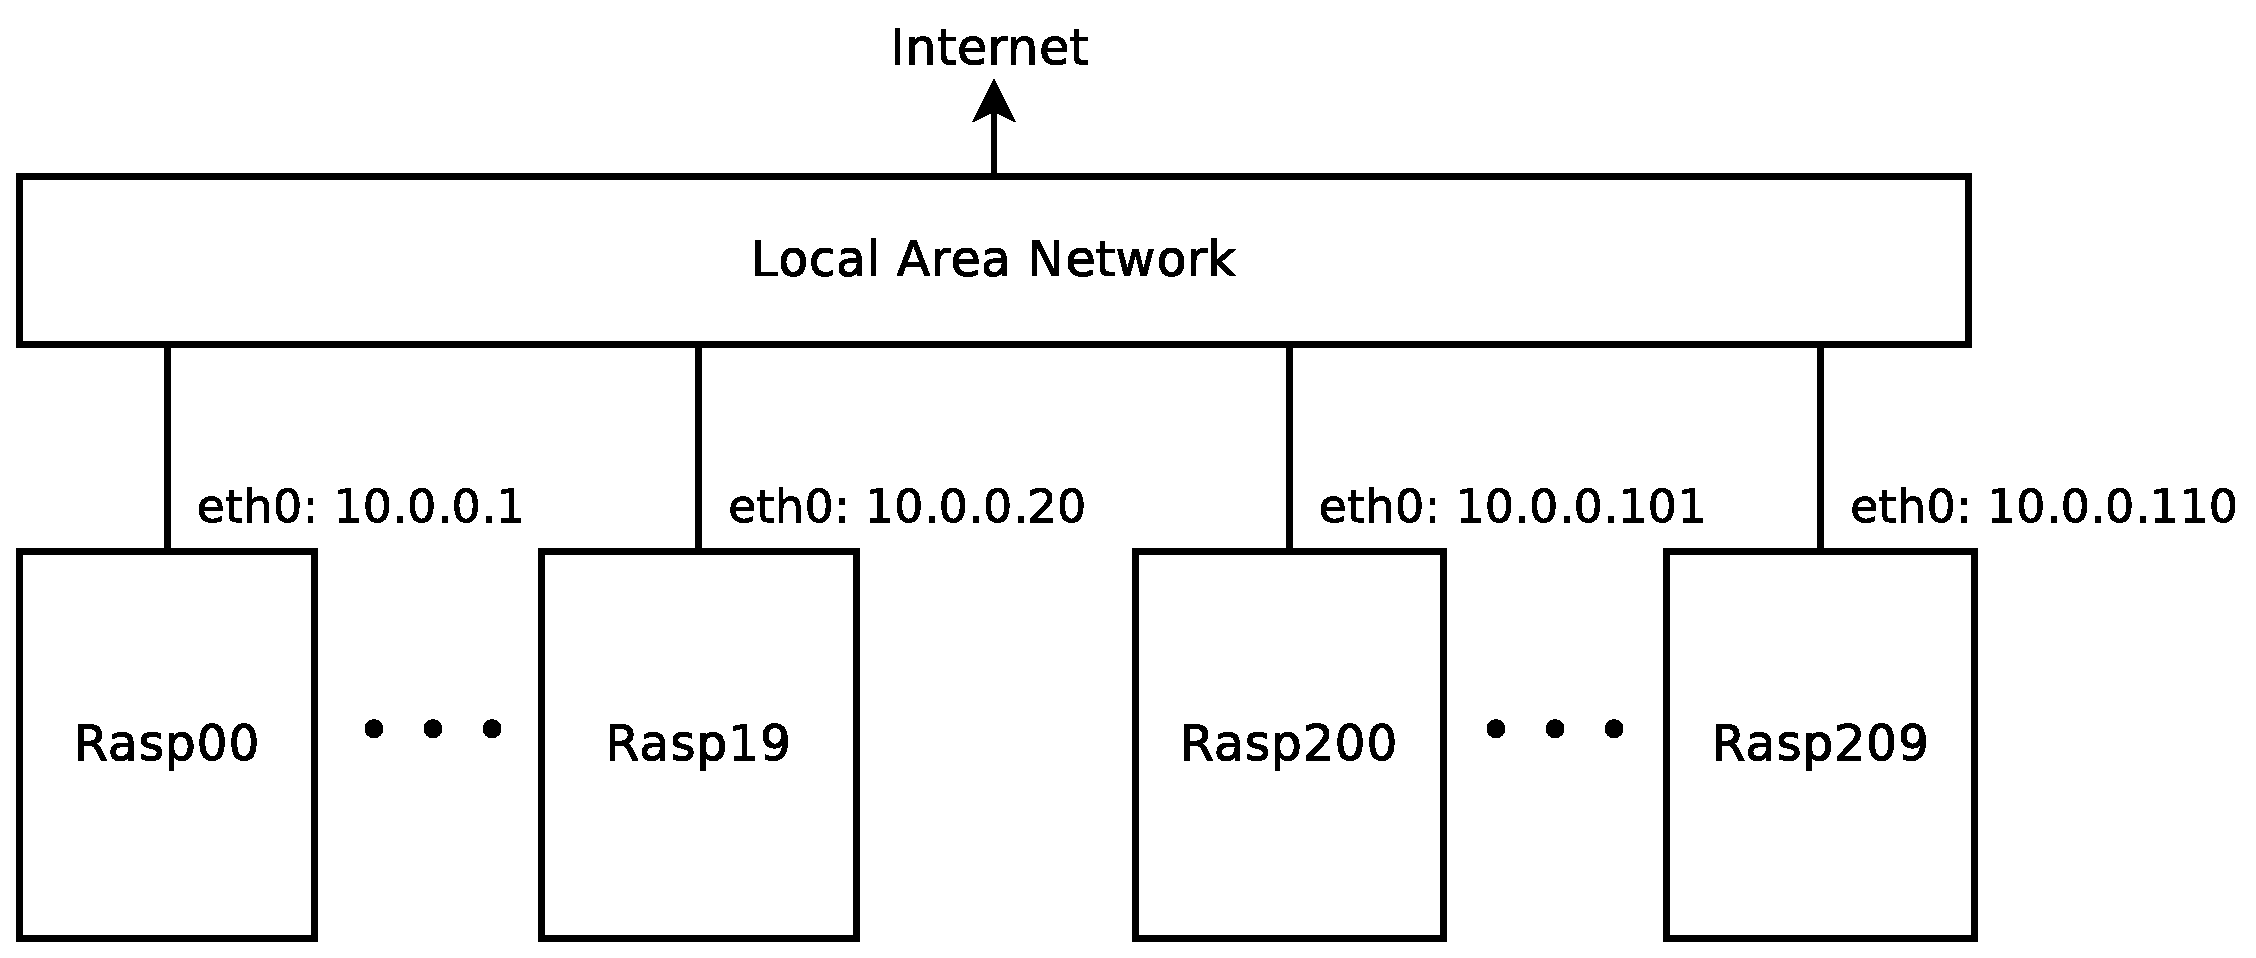
\includegraphics[width=0.6\textwidth]{images/testbed_setup.eps}
\caption{Testbed setup}
\label{fig:testbed_setup}
\end{figure}

We use standard usb power adapters to power the Raspberry Pis.

\subsubsection{Installing Raspbian}

To get started, we first need to install an \ac{OS} on the
Raspberry Pis. We will use Raspbian linux~\cite{raspbian}

We will use a desktop that has linux installed to download,
configure, and write the image to the memory cards.
%We have decided to use a linux desktop machine to create a
%common image of Raspbian Linux that can be used in any of the Raspberry Pis.

%for all devices. After the image has been configured it can be written to
%a memory card and used in any of the Raspberry Pis. This means that each
%device needs a memory card, but it does not matter which card is put into
%which device.

We have decided to go with Raspbian linux~\cite{raspbian} and
to install it on memory cards.


%There exists a number of ways to setup a testbed in a centralized manner.
%E.g. using e.g. \ac{NFS}.

There exists a number of ways to setup a testbed 

with multiple devices. We
have decided on a very simple approach of simply instal


- 
- Download image (wget)
- Update/Modify image (chroot)
- Burn image
- Bang! linux is running
- 


\begin{lstlisting}[frame=single]  % Start your code-block
IMAGE="raspbian_lite-2016-05-31/2016-05-27-raspbian-jessie-lite"
WORKDIR="${HOME}/Raspbian"
cd ${WORKDIR}
wget http://downloads.raspberrypi.org/raspbian_lite/images/${IMAGE}.zip
unzip ${IMAGE}
\end{lstlisting}
\FloatBarrier



We have installed the official Raspbian linux \ac{OS} on all the devices.



\subsection{Installation and Updating}
\subsection{Kodo cross-compilation: From your PC to the Raspberry Pi}

Besides the previous description (\textbf{Include compiling Kodo from the
RasPi from the scratch}), the testbed administrator can compile Kodo in its
personal workstation and transfer the generated binaries directly to
a path in the Raspberry Pi. To achieve this, we get a toolchain that
contains the binaries for the \texttt{raspberry-gxx49-arm-g++} compiler
for the Raspberry Pi. Therefore, we strongly recommend any testbed
administrator to do the following procedure. In what follows, we provide
the instructions considering that the NFS server uses the \texttt{\$HOME}
directory as the working directory. However, the administrator may choose
some other working directory of its preference if desired.

\begin{enumerate}

\item Download the Raspberry Pi toolchain for 64-bit Linux from: \\
\texttt{http://buildbot.steinwurf.dk/toolchains/linux/} to your
\texttt{\$HOME} directory. \\

\item Extract the downloaded file locally in the NFS server. After
this operation, there should be a new directory for the toolchain
in the server. \\

\item Add the \texttt{bin} folder of the toolchain to the \texttt{PATH}
Linux environment variable of the server. This will help the server OS
to recognize the location of the compiler command, which will be needed
later. To do so, edit the \texttt{\$HOME/.profile} to add in a newline:
\texttt{PATH="\$PATH:\$HOME/raspberry-gxx49-arm/bin"}. Save the
\texttt{\$HOME/.profile}. \\

\item Restart the server session in order for the changes made in the
previous step take effect. To verify this, open a new terminal and type:
\texttt{raspberry-gxx49-arm-g++ --version}. A correct binary installation
should return an output similar to:

\texttt{raspberry-gxx49-arm-g++ (crosstool-NG 1.21.0) 4.9.3 20150311 (prerelease)
Copyright (C) 2014 Free Software Foundation, Inc.
This is free software; see the source for copying conditions.  There is NO
warranty; not even for MERCHANTABILITY or FITNESS FOR A PARTICULAR PURPOSE.} \\

\item Clone the Kodo repository in the server by executing: \\
\texttt{git clone git://github.com/steinwurf/kodo.git} in \texttt{\$HOME}. \textbf{Change the repo to kodo-rlnc or kodo-cpp since just raw kodo is going to be depreceated soon} \\

\item Navigate to the repository and configure \texttt{waf} by typing:
\texttt{python config.py} and select the 16th ``make specification'' file
for the Raspberry Pi, e.g. option \texttt{[16]cxx\_raspberry\_gxx49\_arm}
presented by the file.

This command configures \texttt{waf} to use the proper compiler and its
required flags to generate the binaries for the Raspberry Pi. If the
configuration was correct, the output will indicate:
\texttt{'configure' finished successfully (X.XXXs)}, where \texttt{X.XXX}
is total time in seconds for configuring the project in the server. \\

\item Execute \texttt{python waf build}. If the build process was
successful, the generated binaries for the Raspberry Pi should be located
in \texttt{build/cxx\_raspberry\_gxx49\_arm} in the Kodo repository.
\textbf{Indicate how the binary files should look like}.

Once this procedure is made, the testbed administrator can relocate the
generated binary files to Raspberry Pi's through the network as desired
by using the \texttt{scp} command during the configuration step.


\end{enumerate}

\subsection{Kodo Builds for the Raspberry Pi, Platform Support and Documentation}

You can check the build status of Kodo, Fifi and other relevant projects through
their respective repository master branch on our buildbot page
\cite{steinwurf2016buildbot}. Our buildbot displays the status of the builds for
Raspbian 8 and GCC 4.9 for the ARM architecture which is the relevant one for the
Raspberry Pi. At the link, you can check build status and build statistics. Also,
documentation about Kodo basics with a tutorial is available at \cite{kododocs}.

%\label{sec:testbed_nfs}


\subsection{NFS}


\begin{lstlisting}[]
# export NFSBOOTIMAGE="${WORKDIR}/nfsboot"
# export NFSROOTIMAGE="${WORKDIR}/nfsroot"
\end{lstlisting}
\FloatBarrier
\vspace{-5mm}

Extract root partition from image
\begin{lstlisting}[]
# export DEV=$(sudo losetup --show -f -P ${IMAGE}.img); echo $DEV
# dd if=${DEV}p1 of=${NFSBOOTIMAGE}.img bs=4M
# dd if=${DEV}p2 of=${NFSROOTIMAGE}.img bs=4M
\end{lstlisting}
\FloatBarrier
\vspace{-5mm}


Mount nfs root, boot, and home directories
\begin{lstlisting}[]
$ export NFSROOTDIR="${WORKDIR}/nfsroot"
$ mkdir -p ${NFSROOTDIR}
# mount ${NFSROOTIMAGE}.img ${NFSROOTDIR}
# mount ${NFSBOOTIMAGE}.img ${NFSROOTDIR}/boot
\end{lstlisting}
\FloatBarrier
\vspace{-5mm}


Add the below to NFSROOTDIR/boot/cmdline.txt
\begin{lstlisting}[]
ip=dhcp root=/dev/nfs nfs-options=hard,intr,ro
\end{lstlisting}
\FloatBarrier
\vspace{-5mm}


\Suppressnumber\begin{lstlisting}[]
<@\textcolor{gray}{\$\{NFSROOTDIR\}/etc/initramfs-tools/hooks/hooks-rootimg}@>
<@\textcolor{gray}{
---------------------------------------------------------------}
\Reactivatenumber @>
#!/bin/sh

. /usr/share/initramfs-tools/scripts/functions
. /usr/share/initramfs-tools/hook-functions

copy_exec /sbin/losetup
\end{lstlisting}
\FloatBarrier
\vspace{-5mm}


\Suppressnumber\begin{lstlisting}[]
<@\textcolor{gray}{\$\{NFSROOTDIR\}/etc/initramfs-tools/hooks/init-premount-rootimg}@>
<@\textcolor{gray}{
---------------------------------------------------------------}
\Reactivatenumber @>
#!/bin/sh

PREREQ=""
prereqs()
{
   echo "$PREREQ"
}

case $1 in
prereqs)
   prereqs
   exit 0
   ;;
esac

. /scripts/functions
log_begin_msg "Starting rootimg"
log_end_msg

# Setup loop device
losetup /dev/loop0 /imgdir/root.img
\end{lstlisting}
\FloatBarrier
\vspace{-5mm}














IS SETTING UP THE SD-CARD REALLY THE SAME PROCEDURE AS FOR A LOCAL FILESYSTEM?

% Define variable
% export IMAGE="2016-05-27-raspbian-jessie-lite"
% export WORKDIR="${HOME}/Raspbian"
\begin{lstlisting}[]
$ export NFSDEV="/dev/mmcblk0"
\end{lstlisting}
\FloatBarrier
\vspace{-5mm}

\begin{lstlisting}[]
<@\Suppressnumber @># (echo o;                                      # Create DOS partition table
    echo n; echo p; echo 1; echo ; echo +64M;   # Create boot partition
    echo t; echo b;                             # Set boot partition type to FAT
    echo n; echo p; echo 2; echo ; echo ;       # Create home partition
    echo w                                      # Write table to disk
    ) | sudo fdisk ${NFSDEV} <@\Reactivatenumber @>
\end{lstlisting}
\FloatBarrier
\vspace{-5mm}

Print partition table (SHOULD THE BOOT FLAG HAVE BEEN SET TO PARTITION P1?)
\begin{lstlisting}[]
# fdisk -u sectors -l ${NFSDEV}
Disk /dev/mmcblk0: 3.7 GiB, 3965190144 bytes, 7744512 sectors
Units: sectors of 1 * 512 = 512 bytes
Sector size (logical/physical): 512 bytes / 512 bytes
I/O size (minimum/optimal): 512 bytes / 512 bytes
Disklabel type: dos
Disk identifier: 0x00e61b04

Device         Boot  Start     End Sectors  Size Id Type
/dev/mmcblk0p1        2048  133119  131072   64M  b W95 FAT32
/dev/mmcblk0p2      133120 7744511 7611392  3.6G 83 Linux
\end{lstlisting}
\FloatBarrier
\vspace{-5mm}

Format partitions (CONSIDER BTRFS WITH COMPRESSION TO REDUCE ROOT IMAGE SIZE
FOR FASTER BOOT AND LESS BANDWIDTH REQUIREMENTS)
\begin{lstlisting}[]
# mkfs.vfat -n BOOT ${NFSDEV}p1
# mkfs.ext4 -L HOME ${NFSDEV}p2
\end{lstlisting}
\FloatBarrier
\vspace{-5mm}



%Mount image:
%\begin{lstlisting}[]
%# export DEV=$(sudo losetup --show -f -P ${IMAGE}.img); echo $DEV
%# mount ${DEV}p2 ${ROOTDIR}
%# mount ${DEV}p1 ${ROOTDIR}/boot
%\end{lstlisting}
%\FloatBarrier
%\vspace{-5mm}





Copy boot directory:
\begin{lstlisting}[]
# cp -r ${ROOTDIR}/boot/* ${NFSBOOTDIR}/ 
\end{lstlisting}
\FloatBarrier
\vspace{-5mm}



Prepare home directory (Maybe it is better just to copy the content in home from the
image's root partition):
\begin{lstlisting}[]
# install -d -o 1000 -g 1000 -m 700 ${HOMEDIR}/pi && sync
\end{lstlisting}
\FloatBarrier
\vspace{-5mm}



\begin{lstlisting}[]
# mount ${NFSDEV}p1 ${NFSROOTDIR}/boot
# mount ${NFSDEV}p2 ${NFSROOTDIR}/home
\end{lstlisting}
\FloatBarrier
\vspace{-5mm}


Unmount directories:
\begin{lstlisting}[]
# umount ${NFSBOOTDIR} ${NFSHOMEDIR}
\end{lstlisting}
\FloatBarrier
\vspace{-5mm}


\label{sec:testbed_http}
Creating manual copies of the customized image for each memory card can
be also a time-consuming task that is prone to errors and become
cumbersome. Therefore, we present an optional more advanced \ac{HTTP}
image fetching setup for the existing image to be downloaded from a
\ac{HTTP} server. We consider this an optional step since a testbed
administrator might opt for not including this as part of his / her setup.

At the end of Section~\ref{sec:overlay_fs}, the final customized image was
proposed to be splitted into three partitions. One for the boot files, one
containing the root file system and one for the home directory. This is made
considering an overlay filesystem approach. In this section, instead of
writing the image directly to the memory cards, we present how the
partitions can be extracted from the image, and how the boot partition can
be configured to download the root filesystem and home directory partitions
from a \ac{HTTP} server during startup. The advantage of this setup is that
we completely automate the image fetch which significantly eases its
maintainance since any changes are required to be made only in the \ac{HTTP}
server image. We start by declaring the variables for the path names of each
partition:

\begin{lstlisting}[]
$ export HTTPBOOTIMAGE="${WORKDIR}/httpboot"
$ export HTTPROOTIMAGE="${WORKDIR}/httproot"
$ export HTTPHOMEIMAGE="${WORKDIR}/httphome"
\end{lstlisting}
\FloatBarrier
\vspace{-5mm}

We set loopback devices for each of the image partitions and use \texttt{dd} to
extract them from the image:
\begin{lstlisting}[]
# export DEV=$(sudo losetup --show -f -P ${IMAGE}.img); echo $DEV
# dd if=${DEV}p1 of=${HTTPBOOTIMAGE}.img bs=4M
# dd if=${DEV}p2 of=${HTTPROOTIMAGE}.img bs=4M
# dd if=${DEV}p3 of=${HTTPHOMEIMAGE}.img bs=4M
# losetup -d ${DEV}
\end{lstlisting}
\FloatBarrier
\vspace{-5mm}

Now, we configure each of these partitions. The content of the boot image is
copied and modified just once into a memory card and the root
and home images is uploaded to a \ac{HTTP} server. Even though we still
have to manually configure and set the memory cards, we only have
to make this one time, since the \ac{Raspi}s will fetch the root filesystem
from the \ac{HTTP} server every they are turned on.

Create a mountpoint and mount the http root and boot images:
%Mount the http root image and home directories
\begin{lstlisting}[]
$ export HTTPROOTDIR="${WORKDIR}/httproot"
$ mkdir -p ${HTTPROOTDIR}
# mount -o loop ${HTTPROOTIMAGE}.img ${HTTPROOTDIR}
# mount -o loop ${HTTPBOOTIMAGE}.img ${HTTPROOTDIR}/boot
\end{lstlisting}
\FloatBarrier
\vspace{-5mm}

In a previous steps, the boot loader was configured to call an initial \ac{RAM}
filesystem. Now, we present how to the initial \ac{RAM}
filesystem can be extended further to download and cache the root filesystem
from a \ac{HTTP} server before mounting it.

The initial \ac{RAM} filesystem contains an \texttt{init} script that
sets up the prepares the yis first
called. This script initializes the  may be rewritten, but

Create the following file (THE READ-ONLY OPTION IS STILL NOT CONFIGURABLE IN THIS SCRIPT)
\Suppressnumber\begin{lstlisting}[]
<@\textcolor{gray}{\$\{HTTPROOTDIR\}/etc/initramfs-tools/scripts/http}@>
<@\textcolor{gray}{
---------------------------------------------------------------}
\Reactivatenumber @>
# Fetch, cache, and mount root image using HTTP

# Create mount point directory
[ -d /imagedir ] || mkdir /imagedir

# Parse additional command line options
for x in $(cat /proc/cmdline); do
    case $x in
    image=*)
        IMAGE=${x#image=}
        # Extract device and path
        # E.g. /dev/mmcblkp2:/root.img --> /dev/mmcblkp2 and /imagedir/root.img
        IMAGEDEV=${IMAGE%:*}
        IMAGEPATH="${IMAGE#*:}"
        IMAGEPATH="/imagedir/${IMAGEPATH#/}"
        ;;
    url=*)
        URL=${x#url=}
        URL=${URL%/}  # If url has trailing slash, then remove it
        ;;
    esac
done

# Check if variables are declared
[ -z "${IMAGE}" ] && echo "Error: Please add 'image' in cmdline.txt" && exit 1
[ -z "${URL}" ] && echo "Error: Please add 'url' in cmdline.txt" && exit 1

# Fetch and cache root image
http_fetch_image()
{
    configure_networking

    # Fetch list of root image names
    if ! wget -O /tmp/image.csv "${URL}/image.csv"; then
        echo "WARNING failed to fetch image list"
        return
    fi

    # Extract name of image to download based on eth0 MAC
    mac=$(cat /sys/class/net/eth0/address)
    img=$(grep $mac /tmp/image.csv | cut -f2 -d' ')

    # If the image is not cached, then get it
    if [ ! -f "${IMAGEPATH%/*}/${img}" ] && wget --spider -q "${URL}/${img}"; then
        # Delete old image
        rm -f $(readlink -f ${IMAGEPATH})

        # Fetch new image
        if wget -O "${IMAGEPATH%/*}/${img}" "${URL}/${img}"; then
            # If success, create symbolic link to new image
            ln -f -s "${IMAGEPATH%/*}/${img}" ${IMAGEPATH}
        fi
    fi

    # Cleanup
    #rm /tmp/image.csv
}

http_mount_root()
{
    modprobe ext4

    # Mount imagedir
    #mount -n -t ext4 ${IMAGEDEV} /${${IMAGEPATH#/}%%/*}
    mount -n -t ext4 ${IMAGEDEV} /imagedir

    # Fetch and cache root image
    http_fetch_image

    # Mount root as readonly
    losetup /dev/loop0 $(readlink -f ${IMAGEPATH})
    mount -r -n -t ext4 -o nodiratime,noatime /dev/loop0 /root

    # Bind /root/home to /home
    #mount -n -o rbind /home /root/home
}

mountroot()
{
    http_mount_root
}
\end{lstlisting}
\FloatBarrier
\vspace{-5mm}

Make the script executable
\begin{lstlisting}[]
# chmod +x ${HTTPROOTDIR}/etc/initramfs-tools/scripts/http
\end{lstlisting}
\FloatBarrier
\vspace{-5mm}

Keep the content in \texttt{cmdline.txt}, but add/modify the variables
\texttt{boot}, \texttt{ip}, \texttt{image}, \texttt{root}, and \texttt{url}.

%Keep also all other variables as they are in
%\texttt{cmdline.txt}.

%Add the below configurations to \$\{HTTPROOTDIR\}/boot/cmdline.txt
(remove init=/usr/lib/raspi-config/init\_resize.sh earlier in guide)
\Suppressnumber\begin{lstlisting}[]
<@\textcolor{gray}{\$\{HTTPROOTDIR\}/boot/cmdline.txt}@>
<@\textcolor{gray}{
---------------------------------------------------------------}
\Reactivatenumber @>
<@\Suppressnumber @>boot=http ip=dhcp image=/dev/mmcblk0p2:/httproot.img root=/dev/loop0
    url=http://kom.aau.dk/project/TuneSCode/raspi/<@\Reactivatenumber @>
\end{lstlisting}
\FloatBarrier
\vspace{-5mm}
% ip=dhcp root=/dev/http http-options=hard,intr,ro

Here is how the variables are used in the initramfs:
\begin{itemize}
    \item boot=http: tells the init script in initramfs to call the \texttt{http} script presented above
    \item ip=dhcp: use \ac{DHCP} to obtain an \ac{IP} address in the initial ram filesystem
    \item image=<device>:<root image path>: is where the \ac{Raspi} will store the downloaded root image.
    \item root=/dev/loop0: The \texttt{http} initramfs script will make the root filesystem available on /dev/loop0
    \item url=<URL to root image>: Is the directory on a \ac{HTTP} server where the root image will be iavailable.
\end{itemize}


%The \ac{URL} should be modified to reflect where
%the \ac{Raspi}s should download the http root image. The \texttt{image} variable informs the
%\texttt{http} initramfs script to download and cache the http root image in the second partition
%on its memory card at path \texttt{/httproot.img}.



Edit fstab to look like this (exclude the last line if a persistent
home storage directory is not desired):
\Suppressnumber\begin{lstlisting}[]
<@\textcolor{gray}{\$\{HTTPROOTDIR\}/etc/fstab}@>
<@\textcolor{gray}{
---------------------------------------------------------------}
\Reactivatenumber @>
proc            /proc           proc    defaults          0       0
/dev/mmcblk0p1  /boot           vfat    defaults          0       2
/dev/loop0      /               ext4    defaults,noatime  0       1
/dev/mmcblk0p2  /home           ext4    defaults,noatime  0       0
\end{lstlisting}
\FloatBarrier
\vspace{-5mm}


Chroot into the image
% CHROOT to OS image
\begin{lstlisting}[]
$ cd $HTTPROOTDIR
# mount -t proc proc proc/
# mount --bind /sys sys/
# mount --bind /dev dev/
# mount --bind /dev/pts dev/pts
# proot -q qemu-arm-static -S ${HTTPROOTDIR}
# export PS1="(chroot) $PS1"
\end{lstlisting}
\FloatBarrier
\vspace{-5mm}


Create new initramfs (remember that your kernel might be different)
\begin{lstlisting}[]
(chroot) # mkinitramfs -o /boot/init.gz -k 4.4.13+
(chroot) # mkinitramfs -o /boot/init-v7.gz -k 4.4.13-v7+
\end{lstlisting}
\FloatBarrier
\vspace{-5mm}

Exit chroot
\begin{lstlisting}[]
(chroot) # exit
\end{lstlisting}
\FloatBarrier
\vspace{-5mm}

Unmount:
\begin{lstlisting}[]
$ cd ..
# umount ${HTTPROOTIMAGE}/{dev/pts,proc,sys,dev}
\end{lstlisting}
\FloatBarrier
\vspace{-5mm}


\subsection{Prepare sd-card}

IS SETTING UP THE SD-CARD REALLY THE SAME PROCEDURE AS FOR A LOCAL FILESYSTEM?

% Define variable
% export IMAGE="2016-05-27-raspbian-jessie-lite"
% export WORKDIR="${HOME}/Raspbian"
\begin{lstlisting}[]
$ export HTTPDEV="/dev/mmcblk0"
\end{lstlisting}
\FloatBarrier
\vspace{-5mm}

MAYBE ALSO SET THE BOOT FLAG FOR FIRST PARTITION. ALSO UPDATE SCRIPT IF THIS
WORKS. THERE MAY HAVE TO BE ECHOED A 1 AFTER echo a FOR SETTING BOOT FLAG
\begin{lstlisting}[]
<@\Suppressnumber @># (echo o;                                      # Create DOS partition table
    echo n; echo p; echo 1; echo ; echo +64M;   # Create boot partition
    echo t; echo b;                             # Set boot partition type to FAT
    echo a;                                     # Set boot flag
    echo n; echo p; echo 2; echo ; echo ;       # Create home partition
    echo w                                      # Write table to disk
    ) | sudo fdisk ${HTTPDEV} <@\Reactivatenumber @>
\end{lstlisting}
\FloatBarrier
\vspace{-5mm}

Print partition table (SHOULD THE BOOT FLAG HAVE BEEN SET TO PARTITION P1?)
\begin{lstlisting}[]
# fdisk -u sectors -l ${HTTPDEV}
Disk /dev/mmcblk0: 3.7 GiB, 3965190144 bytes, 7744512 sectors
Units: sectors of 1 * 512 = 512 bytes
Sector size (logical/physical): 512 bytes / 512 bytes
I/O size (minimum/optimal): 512 bytes / 512 bytes
Disklabel type: dos
Disk identifier: 0x00e61b04

Device         Boot  Start     End Sectors  Size Id Type
/dev/mmcblk0p1        2048  133119  131072   64M  b W95 FAT32
/dev/mmcblk0p2      133120 7744511 7611392  3.6G 83 Linux
\end{lstlisting}
\FloatBarrier
\vspace{-5mm}

Format partitions
\begin{lstlisting}[]
# mkfs.vfat -n BOOT ${HTTPDEV}p1
# mkfs.ext4 -L HOME ${HTTPDEV}p2
\end{lstlisting}
\FloatBarrier
\vspace{-5mm}






Mount the boot partition from the memory card. Copy the content from the
boot image and unmount it again:
\begin{lstlisting}[]
# mount ${HTTPDEV}p1 ${HTTPROOTDIR}/mnt
# cp -rp ${HTTPROOTDIR}/boot/* ${HTTPROOTDIR}/mnt/ && sync
# umount ${HTTPROOTDIR}/mnt
\end{lstlisting}
\FloatBarrier
\vspace{-5mm}

Mount the home partition from the memory card. Copy the content from the
root image and unmount it again:
\begin{lstlisting}[]
# mount ${HTTPDEV}p2 ${HTTPROOTDIR}/mnt
# cp -rp ${HTTPROOTDIR}/home/* ${HTTPROOTDIR}/mnt/ && sync
# umount ${HTTPROOTDIR}/mnt
\end{lstlisting}
\FloatBarrier
\vspace{-5mm}


\begin{lstlisting}[]
# umount --recursive ${HTTPROOTDIR}
\end{lstlisting}
\FloatBarrier
\vspace{-5mm}


\subsection{Compressing root image (Optional)}

PROBABLY A BETTER IDEA TO USE BTRFS TRANSPARENT COMPRESSION

\begin{lstlisting}[]
# apt-get install squashfs-tools
# mount -o loop ${HTTPROOTIMAGE}.img ${HTTPROOTDIR}
# mksquashfs ${HTTPROOTDIR} compressed_${HTTPROOTIMAGE}.img
\end{lstlisting}
\FloatBarrier
\vspace{-5mm}

\subsection{Try it out}

Upload the root image (\$\{HTTPROOTIMAGE\}.img) to the HTTP server used in the
configurations above. Then, unplug the memory card from the computer.
Insert it into a \ac{Raspi} and
turn it on. It is recommended that the \ac{Raspi} is turned on with a monitor
connected the first time the newly created Linux installation is tested to
assure that Raspbian starts up correctly.


PRESENT FILES ON HTTP. E.G. HTTPROOT.IMG AND IMAGES.CSV


\begin{itemize}
    \item Copy http root image (\$\{HTTPROOTIMAGE\}.img) a HTTP server
    \item Create images.csv
\end{itemize}


\Suppressnumber\begin{lstlisting}[]
<@\textcolor{gray}{http://<SERVERIP>/.../images.csv}@>
<@\textcolor{gray}{
---------------------------------------------------------------}
\Reactivatenumber @>
# Ethernet MAC    Root image
b8:27:eb:5b:da:20 httproot_1.img
b8:27:eb:7b:c3:91 httproot_1.img
b8:27:eb:7b:c3:91 httproot_2.img
...
\end{lstlisting}
\FloatBarrier
\vspace{-5mm}

Notice that the \ac{Raspi}s can be configured to download different root images.
This is useful both for having various root images for subsets of the \ac{Raspi}s,
but also as a basic way inform the \ac{Raspi}s that the root image changed such
that they can download the new root image at next boot.

As of this writing, there is unfortunately a bug in wget that makes wget not showing
its progress bar while downloading the root image at startup. Instead, it may appear
to be unable to connect although it is downloading, so keep patient.

\begin{lstlisting}[]
Connecting to <HTTP SERVER IP> (<HTTP SERVER IP>:<PORT>)
image.csv       100% |*******************************************************| 1287   0:00:00 ETA
Connecting to <HTTP SERVER IP> (<HTTP SERVER IP>:<PORT>)
_
\end{lstlisting}
\FloatBarrier
\vspace{-5mm}


REMEMBER TO COPY-PASTE ALL CONTENT FROM SCRIPT INTO LATEX AGAIN IN CASE SOME
SCRIPT CHANGED, BUT WAS NOT UPDATED IN LATEX


\section{Cross-compilation: From PC to Raspberry Pi}

%\subsection{Kodo cross-compilation: From your PC to the Raspberry Pi}

Modern \ac{PC}s are significantly better equipped than the \ac{Raspi}s that in
contrasts to \ac{PC}s target a far more affortable and smaller module size. This
means that it may be preferred or even mandatory to perform some computational
expensive tasks in a \ac{PC} rather than in \ac{Raspi}s.
Example of tasks that are quite computational expensive is to compile software
packages and large libraries.
Another reason to use a \ac{PC} may be the hardware limitations of \ac{Raspi}s
in terms of e.g. memory and disk space. Some software packages might simply be
too memory demanding to be compiled in a \ac{Raspi}.
Thus, this section will present how to setup a toolchain in a \ac{PC} that can
be used to cross compile C++ code to the ARM architecture that the \ac{Raspi}s.
The toolchain is mandatory on most consumer \ac{PC}s due to the different
processor architecture.

Furthermore, we will cover how to cross compile a simple C++ example and
Kodo-cpp as well as how the binaries can be copied from a \ac{PC} to a
\ac{Raspi} and executed.
There exists bindings to Kodo in various programming language. We will present
how to also run a Kodo-python application in a \ac{Raspi}.

%WRITE INTRO OF WHY WE WANT TO CROSS COMPILE. E.G. 1) WE DO NOT HAVE MONITORS
%CONNECTED TO THE RASPIS, 2) A PC IS SIGNIFICANTLY FASTER AND FAR BETTER EQUIPPED (RAM, CPU, HARDDRIVE), 3) MORE CONVINIENT TO DO EVERYTHING IN ONE PC AND DISTRIBUTE IT TO THE RASPIS AFTERWARDS. MORE?

\subsection{Install toolchain on PC}

%Besides the previous description (\textbf{Include compiling Kodo from the
%RasPi from the scratch}), the testbed administrator can compile Kodo in its
%personal workstation and transfer the generated binaries directly to
%a path in the \ac{Raspi}. To achieve this, we get a toolchain that
%contains the binaries for the \texttt{raspberry-gxx49-arm-g++} compiler
%for the \ac{Raspi}. Therefore, we strongly recommend any testbed
%administrator to do the following procedure. In what follows, we provide
%the instructions considering that the NFS server uses the \texttt{\$HOME}
%directory as the working directory. However, the administrator may choose
%some other working directory of its preference if desired.

\begin{enumerate}

\item Create toolchain directory:
\begin{lstlisting}[]
$ TOOLCHAINDIR="${HOME}/toolchains"
$ mkdir -p $TOOLCHAINDIR
$ cd $TOOLCHAINDIR
\end{lstlisting}
\FloatBarrier
\vspace{-5mm}

\item Download the \ac{Raspi} toolchain for 64-bit Linux from.
A more recent \ac{Raspi} toolchain may be available at
\texttt{http://buildbot.steinwurf.dk/toolchains/linux/}:

\begin{lstlisting}[]
$ TOOLCHAIN="raspberry-gxx49-arm"
$ wget http://kom.aau.dk/project/TuneSCode/raspi/${TOOLCHAIN}.zip
\end{lstlisting}
\FloatBarrier
\vspace{-5mm}

\item Extract the downloaded file:
%locally in the NFS server. After
%this operation, there should be a new directory for the toolchain
%in the server. \\
\begin{lstlisting}[]
$ unzip ${TOOLCHAIN}.zip
\end{lstlisting}
\FloatBarrier
\vspace{-5mm}

\item (Optional) Delete zip file:
%locally in the NFS server. After
%this operation, there should be a new directory for the toolchain
%in the server. \\
\begin{lstlisting}[]
$ rm ${TOOLCHAIN}.zip
\end{lstlisting}
\FloatBarrier
\vspace{-5mm}

\item We can now verify that the ARM cross compiler is working:

\begin{lstlisting}[]
$ ${TOOLCHAINDIR}/${TOOLCHAIN}/bin/${TOOLCHAIN}-g++ --version
raspberry-gxx49-arm-g++ (crosstool-NG 1.21.0) 4.9.3 20150311 (prerelease)
Copyright (C) 2014 Free Software Foundation, Inc.
This is free software; see the source for copying conditions.  There is NO
warranty; not even for MERCHANTABILITY or FITNESS FOR A PARTICULAR PURPOSE.
\end{lstlisting}
\FloatBarrier
\vspace{-5mm}

%\begin{lstlisting}[]
%$ echo "${TOOLCHAINDIR}/${TOOLCHAIN}/bin/${TOOLCHAIN}-g++"
%/home/<USER>/toolchains/raspberry-gxx49-arm/bin/raspberry-gxx49-arm-g++
%\end{lstlisting}
%\FloatBarrier
%\vspace{-5mm}
    
%    The ARM cross compilers should now be located in

\item Make toolchain binaries available systemwide. Instead of calling
the ARM cross compiler using its full path, we can make it accessible
from the command shell systemwide. One way to do this is by adding the 
toolchain binaries directory to the Linux environment variable \texttt{PATH}
when the \ac{OS} starts up:

%\item Add toolchain binaries to \texttt{PATH}. Instead specifying the full
%path to the toolchain binaries we can instead tell the operation system
%where to search for it. This makes the toolchain binaries available
%systemwide.

\begin{lstlisting}[]
$ echo PATH=\"\$PATH:${TOOLCHAINDIR}/${TOOLCHAIN}/bin\" >> ${HOME}/.profile
\end{lstlisting}
\FloatBarrier
\vspace{-5mm}
%$ printf 'PATH="%s/%s/bin"\n' "${TOOLCHAINDIR}" "${TOOLCHAIN}" >> ${HOME}/.profile

%\item Add the \texttt{bin} folder of the toolchain to the \texttt{PATH}
%Linux environment variable of the server. This will help the server OS
%to recognize the location of the compiler command, which will be needed
%later. To do so, edit the \texttt{\$HOME/.profile} to add in a newline:
%\texttt{PATH="\$PATH:\$HOME/raspberry-gxx49-arm/bin"}. Save the
%\texttt{\$HOME/.profile}. \\

\texttt{.profile} should now contain the line we inserted. There may be more
code in you file.
% MAC and Hostname file
\Suppressnumber\begin{lstlisting}[]
<@\textcolor{gray}{\$HOME/.profile}@>
<@\textcolor{gray}{
---------------------------------------------------------------}
\Reactivatenumber @>
PATH="$PATH:/home/<USERNAME>/toolchains/raspberry-gxx49-arm/bin"
\end{lstlisting}
\FloatBarrier

\item Update \texttt{PATH}. Source \texttt{.profile} to make the changes
take effect in your system:
\begin{lstlisting}[]
$ source ${HOME}/.profile
\end{lstlisting}
\FloatBarrier
\vspace{-5mm}

\item ARM cross compiler should now be available systemwide:

\begin{lstlisting}[]
$ raspberry-gxx49-arm-g++ --version
\end{lstlisting}
\FloatBarrier
\vspace{-5mm}

%\item Restart the server session in order for the changes made in the
%previous step take effect. To verify this, open a new terminal and type:
%\texttt{raspberry-gxx49-arm-g++ --version}. A correct binary installation
%should return an output similar to:
%
%\texttt{raspberry-gxx49-arm-g++ (crosstool-NG 1.21.0) 4.9.3 20150311 (prerelease)
%Copyright (C) 2014 Free Software Foundation, Inc.
%This is free software; see the source for copying conditions.  There is NO
%warranty; not even for MERCHANTABILITY or FITNESS FOR A PARTICULAR PURPOSE.} \\

\end{enumerate}

\subsection{Cross compile example}

The following example will provide a very basic example of 1) how to cross compile
a \texttt{hello\_world} c++ example to the \ac{Raspi}'s ARM architecture
and 2) how to copy and execute the binary in a \ac{Raspi} using \ac{SCP} and \ac{SSH}.

Lets create a directory to hold our code:
\begin{lstlisting}[]
$ CODEDIR="${HOME}/code"
$ mkdir -p ${CODEDIR}
$ cd ${CODEDIR}
\end{lstlisting}
\FloatBarrier
\vspace{-5mm}

Create the file \texttt{hello\_world.cpp} with the following content using your
favorite text editor:

\Suppressnumber\begin{lstlisting}[]
<@\textcolor{gray}{\${CODEDIR}/hello\_world.cpp}@>
<@\textcolor{gray}{
---------------------------------------------------------------}
\Reactivatenumber @>
#include <iostream>

int main()
{
    std::cout << "Hello World!" << std::endl;
    return 0;
}
\end{lstlisting}
\FloatBarrier

Save \texttt{hello\_world.cpp} and compile it for \ac{Raspi}:

\begin{lstlisting}[]
$ raspberry-gxx49-arm-g++ hello_world.cpp -o hello_world
\end{lstlisting}
\FloatBarrier
\vspace{-5mm}

This should produce a binary \texttt{hello\_world}. Copy it to a \ac{Raspi}
and test it. We will use \ac{SCP} to copy the binary file to one of the \ac{Raspi}s.

The default username for our Raspbian lite distribution is "pi" and password is "raspberry"

\begin{lstlisting}[]
$ scp main pi:<RASP_IP>:~/
\end{lstlisting}
\FloatBarrier
\vspace{-5mm}

If you do not know the \ac{IP} address of a \ac{Raspi} in your network, you can
connect a monitor to it and run the following command after you have logged in:
\begin{lstlisting}[]
pi@rasp01:~ $ ifconfig
eth0      Link encap:Ethernet  HWaddr b8:27:eb:72:77:54  
          inet addr:192.168.87.107  Bcast:192.168.87.255  Mask:255.255.255.0
          inet6 addr: fe80::e0a5:38f3:6f82:bc79/64 Scope:Link
          UP BROADCAST RUNNING MULTICAST  MTU:1500  Metric:1
          RX packets:1537 errors:0 dropped:0 overruns:0 frame:0
          TX packets:445 errors:0 dropped:0 overruns:0 carrier:0
          collisions:0 txqueuelen:1000 
          RX bytes:259117 (253.0 KiB)  TX bytes:52551 (51.3 KiB)

\end{lstlisting}
\FloatBarrier
\vspace{-5mm}

After the executable has been copied to a \ac{Raspi}. Then, \ac{SSH} to it:

\begin{lstlisting}[]
$ ssh pi:<RASP_IP>
\end{lstlisting}
\FloatBarrier
\vspace{-5mm}

We can list the directory content after we have logged into the \ac{Raspi} and
see that \texttt{hello\_world} is there:

\begin{lstlisting}[]
pi@rasp07:~ $ ls
hello_world  rasp_config
\end{lstlisting}
\FloatBarrier
\vspace{-5mm}

Now, simply execute the \texttt{hello\_world} to confirm that cross compiling
\texttt{hello\_world} worked properly:

\begin{lstlisting}[]
pi@rasp07:~ $ ./hello_world
Hello World!
\end{lstlisting}
\FloatBarrier
\vspace{-5mm}

\subsection{Cross compile Kodo}

Kodo is a C++11 library for \ac{NC}. There exists a number of bindings for
Kodo to other popular programming languages. This procedure will go through
how to setup Kodo-cpp to cross compile to \ac{Raspi}. Kodo-cpp provides a
simple interface to the underlying C++11 code that exists in the libraries
Kodo-core and Kodo-rlnc.

In order to use Kodo, it is required to obtain a research- and
education-friendly license.
A license can be obtained from \url{http://steinwurf.com/license.html}. It is
free for research and educational purposes.

A more detailed procedure of setting up Kodo-cpp than provided below is available at
\url{http://docs.steinwurf.com/kodo/kodo-cpp/index.html}

\begin{enumerate}

\item Start by creating a directory to hold our code:
\begin{lstlisting}[]
$ CODEDIR="${HOME}/code"
$ mkdir -p ${CODEDIR}
$ cd ${CODEDIR}
\end{lstlisting}
\FloatBarrier
\vspace{-5mm}

\item Clone the Kodo repository and change directory into the repository:
\begin{lstlisting}[]
$ git clone https://github.com/steinwurf/kodo-cpp.git
$ cd kodo-cpp
\end{lstlisting}
\FloatBarrier
\vspace{-5mm}

\item Configure Kodo to build executables for the \ac{ARM} architecture using our toolchain:
\begin{lstlisting}[]
$ python waf configure --cxx_mkspec=cxx_raspberry_gxx49_arm
...
'configure' finished successfully (0.620s)
\end{lstlisting}
\FloatBarrier
\vspace{-5mm}

\item Build executables:
\begin{lstlisting}[]
$ python waf build
...
'build' finished successfully (2m22.918s)
\end{lstlisting}
\FloatBarrier
\vspace{-5mm}


\item Make shared library:
\begin{lstlisting}[]
$ python waf install --install_shared_libs --install_path="./shared_test"
\end{lstlisting}
\FloatBarrier
\vspace{-5mm}

\item Copy shared library to a \ac{Raspi}'s home directory (Alternatively, Kodo can also generate static libraries):
\begin{lstlisting}[]
$ scp -r shared_test/include shared_test/libkodoc.so pi@<RASP_IP>:~/
\end{lstlisting}
\FloatBarrier
\vspace{-5mm}

\item Copy a binary using Kodo shared library to the \ac{Raspi}'s home directory:
\begin{lstlisting}[]
$ scp -r shared_test/encode_decode_simple pi@<RASP_IP>:~/
\end{lstlisting}
\FloatBarrier
\vspace{-5mm}

\item Execute binary:
\begin{lstlisting}[]
$ ssh pi@<RASP_IP> ./encode_decode_simple
Data decoded correctly
\end{lstlisting}
\FloatBarrier
\vspace{-5mm}

Cross compiling Kodo applications works provided that above command
returned "Data decoded correctly".

%\item Navigate to the repository and configure \texttt{waf} by typing:
%\texttt{python config.py} and select the 16th ``make specification'' file
%for the \ac{Raspi}, e.g. option \texttt{[16]cxx\_raspberry\_gxx49\_arm}
%presented by the file.
%
%This command configures \texttt{waf} to use the proper compiler and its
%required flags to generate the binaries for the \ac{Raspi}. If the
%configuration was correct, the output will indicate:
%\texttt{'configure' finished successfully (X.XXXs)}, where \texttt{X.XXX}
%is total time in seconds for configuring the project in the server. \\
%
%\item Execute \texttt{python waf build}. If the build process was
%successful, the generated binaries for the \ac{Raspi} should be located
%in \texttt{build/cxx\_raspberry\_gxx49\_arm} in the Kodo repository.
%\textbf{Indicate how the binary files should look like}.
%
%Once this procedure is made, the testbed administrator can relocate the
%generated binary files to the \ac{Raspi}s through the network as desired
%by using the \texttt{scp} command during the configuration step.


\end{enumerate}

\subsection{Kodo Builds for the \ac{Raspi}, Platform Support and Documentation}

You can check the build status of Kodo, Fifi and other relevant projects
through their respective repository master branch on our buildbot page
\cite{steinwurf2016buildbot}. Our buildbot displays the status of the builds
for Raspbian 8 and GCC 4.9 for the ARM architecture which is the relevant one
for the \ac{Raspi}. At the link, you can check build status and build
statistics. Also, documentation about Kodo basics with a tutorial is available
at \cite{kododocs}.






\subsection{Kodo python}

WRITE HOW TO RUN A KODO PYTHON SCRIPT IN THE RASPIS

\subsection{fabric}

SHORT INTRO. EXPLAIN A FEW USECASES FOR FABRIC. E.G. REBOOT, INSTALL PACKAGE, RUN SCRIPT ON MULTIPLE RASPIS. COPY FILES TO/FROM PC AND MULTIPLE RASPIS 


% Exit chroot, umount, and write to memory card
\begin{lstlisting}[]
from fabric.api import run, env, task
# Python Fabric script to run commands on multiple hosts through ssh
#
# Run script as 'fab <task>', where <task> is one of the scripts functions
# marked as a tesk. The task marked as 'default' will be run if <task> is not
# specified

env.hosts = ['rasp00.domain.com','rasp01.domain.com','rasp02.domain.com']
env.user = 'root'
env.password = 'sdn'

@task
def install(program):
    """
    Install a program
    program: program name
    """
    result = run('apt-get install -y {}'.format(program), quiet=True)

@task
def copy_to_rasp(filename):
    put(...)

\end{lstlisting}
\FloatBarrier

execute a script function by calling "fab install:feh"




\subsection{Long running jobs over SSH (PUT THIS SECTION SOMEWHERE ELSE)}

Problem when you logout, then applications will terminate. SCREEN is the answer.

EXAMPLE

\texttt{hello\_world} returns immediately. This is not always the case.
Sometimes it is desired to run simulations that should run for days. 
A software package called \texttt{screen} can be used for this purpose.
Simply run ...


\section{Conclusion}
\label{sec:conclusions}
Observing the expectation of the \ac{IoT} and lack for a low-cost, easy-to-configure testbed in this area for reproducible research, we provide an in-depth description of the new Aalborg University's \ac{Raspi} testbed for network coding evaluation and how to guarantee replicability and scaling managing of this system. The description shows how to set up interconnected \ac{Raspi}s with memory cards for local storage, a Raspbian Lite image, network connectivity and proper system administration privileges. Using the presented procedure permits to setup a Raspbian Lite for the \ac{Raspi}s, but this restrics the testbed administrators to specifically using this \ac{OS} regardless of the \ac{Raspi} model. Other Linux distributions might be setup with Yocto to create an image from the scratch that are tailored for the \ac{Raspi}, even to specific models. However, that would require to compile the software for the \ac{Raspi} from scratch which can be a tedious angd long task. Still, this method could be adequate for an expert user. We hope this work permits researchers to replicate setups and scenarios for evaluating their strategies in a rapid and manageable way. Future work in the use of \ac{Raspi} devices will focus on expanding the setup and automation of tasks to run the testbed, configure specified network topologies (e.g., with specific connectivity or packet loss ratios), reserve the use of these sub-networks for running tailored experiments and opening the use of the testbed beyond our team at Aalborg University. Future work in this area will consider to make the testbed fetch the image through the \ac{HTTP} server. This is expected to simplify the maintenance of the memory cards.


%%%%%%%%%%%%%%%%%%%%%%%%%%%%%%%%%%%%%%%%%%
% \subsection{Subsection}
% \subsubsection{Subsubsection}

% Bulleted lists look like this:
% \begin{itemize}[leftmargin=*,labelsep=4mm]
% \item	First bullet
% \item	Second bullet
% \item	Third bullet
% \end{itemize}

% Numbered lists can be added as follows:
% \begin{enumerate}[leftmargin=*,labelsep=3mm]
% \item	First item
% \item	Second item
% \item	Third item
% \end{enumerate}

% The text continues here.

% \subsection{Figures, Tables and Schemes}

% All figures and tables should be cited in the main text as Figure 1, Table 1, etc.

% \begin{figure}[H]
% \centering
% %
\includegraphics[width=3cm]{logo-mdpi}
% \caption{This is a figure, Schemes follow the same formatting. If there are multiple panels, they should be listed as: (\textbf{a}) Description of what is contained in the first panel. (\textbf{b}) Description of what is contained in the second panel. Figures should be placed in the main text near to the first time they are cited. A caption on a single line should be centered.}
% \end{figure}

% \begin{table}[H]
% \caption{This is a table caption. Tables should be placed in the main text near to the first time they are cited.}
% \small % Font size can be changed to match table content. Recommend 10 pt.
% \centering
% \begin{tabular}{ccc}
% \toprule
% \textbf{Title 1}	& \textbf{Title 2}	& \textbf{Title 3}\\
% \midrule
% entry 1		& data			& data\\
% entry 2		& data			& data\\
% \bottomrule
% \end{tabular}
% \end{table}

% \subsection{Formatting of Mathematical Components}

% This is an example of an equation:

% \begin{equation}
% \mathbb{S}
% \end{equation}

%% If the documentclass option "submit" is chosen, please insert a blank line before and after any math environment (equation and eqnarray environments). This ensures correct linenumbering. The blank line should be removed when the documentclass option is changed to "accept" because the text following an equation should not be a new paragraph.
% Please punctuate equations as regular text. Theorem-type environments (including propositions, lemmas, corollaries etc.) can be formatted as follows:
%% Example of a theorem:
% \begin{Theorem}
% Example text of a theorem.
% \end{Theorem}
% The text continues here. Proofs must be formatted as follows:

%% Example of a proof:
% \begin{proof}[Proof of Theorem 1]
% Text of the proof. Note that the phrase `of Theorem 1' is optional if it is clear which theorem is being referred to.
% \end{proof}
% The text continues here.

%%%%%%%%%%%%%%%%%%%%%%%%%%%%%%%%%%%%%%%%%%
%\section{Discussion}

%This section may be divided by subheadings. Authors should discuss the results and how they can be interpreted in perspective of previous studies and of the working hypotheses. The findings and their implications should be discussed in the broadest context possible. Future research directions may also be highlighted.

%%%%%%%%%%%%%%%%%%%%%%%%%%%%%%%%%%%%%%%%%%
%\section{Materials and Methods}

%This section should be divided by subheadings. Materials and Methods should be described with sufficient details to allow others to replicate and build on published results. Please note that publication of your manuscript implicates that you must make all materials, data, and protocols associated with the publication available to readers. Please disclose at the submission stage any restrictions on the availability of materials or information. New methods and protocols should be described in detail while well-established methods can be briefly described and appropriately cited.

%Research manuscripts reporting large datasets that are deposited in a publicly available database should specify where the data have been deposited and provide the relevant accession numbers. If the accession numbers have not yet been obtained at the time of submission, please state that they will be provided during review. They must be provided prior to publication.

%%%%%%%%%%%%%%%%%%%%%%%%%%%%%%%%%%%%%%%%%%
%\section{Conclusions}

%This section is not mandatory, but can be added to the manuscript if the discussion is unusually long or complex.

%%%%%%%%%%%%%%%%%%%%%%%%%%%%%%%%%%%%%%%%%%
\vspace{6pt}

%%%%%%%%%%%%%%%%%%%%%%%%%%%%%%%%%%%%%%%%%%
%% optional
% \supplementary{The following are available online at www.mdpi.com/link, Figure S1: title, Table S1: title, Video S1: title.}

%%%%%%%%%%%%%%%%%%%%%%%%%%%%%%%%%%%%%%%%%%
\acknowledgments{This research has been partially financed by the
Marie Curie Initial Training Network (ITN) CROSSFIRE project
(Grant No. EU - FP7 - CROSSFIRE - 317126) from the European Comission FP7
framework, the Green Mobile Cloud project (Grant No. DFF - 0602 - 01372B),
the TuneSCode project (Grant No. DFF - 1335 - 00125) both granted by the
Danish Council for Independent Research (Det Frie Forskningsr\r{a}d), and
by the German Research Foundation (DFG) within the Collaborative Research
Center SFB 912 – HAEC.}

%All sources of funding of the study should be disclosed. Please clearly indicate grants that you have received in support of your research work. Clearly state if you received funds for covering the costs to publish in open access.

%%%%%%%%%%%%%%%%%%%%%%%%%%%%%%%%%%%%%%%%%%
% \authorcontributions{For research articles with several authors, a short paragraph specifying their individual contributions must be provided. The following statements should be used ``X.X. and Y.Y. conceived and designed the experiments; X.X. performed the experiments; X.X. and Y.Y. analyzed the data; W.W. contributed reagents/materials/analysis tools; Y.Y. wrote the paper.'' Authorship must be limited to those who have contributed substantially to the work reported.}

%%%%%%%%%%%%%%%%%%%%%%%%%%%%%%%%%%%%%%%%%%
\conflictofinterests{The authors declare no conflict of interest. The founding sponsors had no role in the design of the study; in the collection, analyses, or interpretation of data; in the writing of the manuscript, and in the decision to publish the results.}

%Declare conflicts of interest or state ``The authors declare no conflict of interest.'' Authors must identify and declare any personal circumstances or interest that may be perceived as inappropriately influencing the representation or interpretation of reported research results. Any role of the funding sponsors in the design of the study; in the collection, analyses or interpretation of data; in the writing of the manuscript, or in the decision to publish the results must be declared in this section. If there is no role, please state ``The founding sponsors had no role in the design of the study; in the collection, analyses, or interpretation of data; in the writing of the manuscript, and in the decision to publish the results''.

%%%%%%%%%%%%%%%%%%%%%%%%%%%%%%%%%%%%%%%%%%
%% optional
\abbreviations{The following abbreviations are used in this manuscript:\\

% Use these two commands to get used acronyms
%used=$(grep -ohR '\\ac{[^}]*' *.tex | cut -f2 -d'{' | sort | uniq)
%for ac in ${used[@]}; do echo "$(grep -R "acro{${ac}}" acronym.tex)"; done | cut -f2-4 -d'{'
% Use text editor to replace '}{' --> ': ' and '}' --> '\\'

\textcolor{red}{
\noindent ACK: Acknowledgment\\
AMR: Adaptive Multi-Rate\\
ARM: Advanced RISC Machine\\
BLAS: Basic Linear Algebra Subprograms\\
CPU: Central Processing Unit\\
CSMA/CA: Carrier Sense Multiple Access with Collision Avoidance\\
GB: Gigabyte\\
D2D: Device to Device\\
DAG: Direct Acyclic Graph\\
DC: Direct Current\\
DCF: Distributed Coordination Function\\
GF: Galois Field\\
GPU: Graphic Processing Unit\\
IP: Internet Protocol\\
IPTV: Internet Protocol TeleVision\\
LAN: Local Area Network\\
l.d.: linearly dependent\\
l.i.: linearly independent\\
LNC: Linear Network Coding\\
LOS: Line Of Sight\\
MAC: Medium Access Control\\
MIMO: Multiple Input Multiple Output\\
NC: Network Coding\\
NLOS: Non Line Of Sight\\
OSI: Open Systems Interconnect\\
PC: Personal Computer\\
PNC: Physical layer Network Coding\\
QoE: Quality of Experience\\
RLNC: Random Linear Network Coding\\
SRLNC: Sparse Random Linear Network Coding\\
SIMD: Single Instruction Multiple Data\\
SIMD: Single Instruction Multiple Data\\
SMP: Symmetric Multiprocessor\\
SOC: System on Chip\\
SSE: Streaming SIMD Extensions\\
TSNC: Tunable Sparse Network Coding\\
VoIP: Voice over Internet Protocol\\
WLAN: Wireless Local Area Network\\
dof: degrees of freedom\\
IP: Internet Protocol\\
OS: Operating System\\
NFS: Network File System\\
RAM: Random Access Memory\\
Raspi: Raspberry Pi\\
SSH: Secure Shell\\
USB: Universal Serial Bus\\
SCP: Secure copy\\
Telnet: Telnet}}

%%%%%%%%%%%%%%%%%%%%%%%%%%%%%%%%%%%%%%%%%%
%% optional
% \appendix
% \section{}
% The appendix is an optional section that can contain details and data supplemental to the main text. For example, explanations of experimental details that would disrupt the flow of the main text, but nonetheless remain crucial to understanding and reproducing the research shown; figures of replicates for experiments of which representative data is shown in the main text can be added here if brief, or as Supplementary data. Mathemtaical proofs of results not central to the paper can be added as an appendix.

% \section{}
% All appendix sections must be cited in the main text. In the appendixes, Figures, Tables, etc. should be labeled starting with `A', e.g., Figure A1, Figure A2, etc.

%%%%%%%%%%%%%%%%%%%%%%%%%%%%%%%%%%%%%%%%%%
\bibliographystyle{mdpi}

%=====================================
% References, variant A: internal bibliography
%=====================================
% \renewcommand\bibname{References}
% \begin{thebibliography}{999}
% % Reference 1
% \bibitem{ref-journal}
% Lastname, F.; Author, T. The title of the cited article. {\em Journal Abbreviation} {\bf 2008}, {\em 10}, 142-149.
% % Reference 2
% \bibitem{ref-book}
% Lastname, F.F.; Author, T. The title of the cited contribution. In {\em The Book Title}; Editor, F., Meditor, A., Eds.; Publishing House: City, Country, 2007; pp. 32-58.
% \end{thebibliography}

%=====================================
% References, variant B: external bibliography
%=====================================
\bibliography{raspi_journal}

%%%%%%%%%%%%%%%%%%%%%%%%%%%%%%%%%%%%%%%%%%
%% optional
\sampleavailability{The testbed and measurements in this publication are both available from the authors.}

%%%%%%%%%%%%%%%%%%%%%%%%%%%%%%%%%%%%%%%%%%
\end{document}
